\chapter{LITERATURE REVIEW}
\label{chapter:literature_review}

\par
The initial phase of the thesis involved getting familiar with concept of \acrshort{mbt}, analyzing previously done or currently ongoing researches and case studies related to \acrshort{mbt} and choosing the right tool which conformed with our requirements through literature review. Within this phase 16 research papers, 1 master's thesis and 1 patent description were read completely, analyzed and documented. Multiple \acrshort{mbt} tools were configured and tried out to find the best suitable one for \acrshort{bsc}. Overall results and highlights can be read in sections below.

\section{Modeling Paradigms}

\par
As the extensive research has been done for already couple of decades related to usage of modeling in software development, this resulted in multiple modeling paradigms available today. Table \ref{tab:Usage_Survey} lists the most popular modeling notations according to a survey on \acrshort{mbt} approaches \cite{Survey}.

\begin{table}[]
    \centering
    \begin{tabular}{|l|r|}
        \hline
        \textbf{Modeling Notations} & \textbf{Usage Amounts} \\
        \hline
        Statechart Diagram & 27 \\
        \hline
        Class Diagram & 19 \\
        \hline
        Sequence Diagram & 19 \\
        \hline
        Use Case Diagram & 11 \\
        \hline
        OCL & 11 \\
        \hline
        (Extended) Finite State Machine & 10 \\
        \hline
        Activity Diagram & 9 \\
        \hline
        Collaboration Diagram & 8 \\
        \hline
        Object Diagram & 7 \\
        \hline
        Graph & 7 \\
        \hline
        Z Specification & 4 \\
        \hline
    \end{tabular}
    \caption{Usage of \acrshort{mbt} notations \cite{Survey}}
    \label{tab:Usage_Survey}
\end{table}

Multiple modeling paradigms are perfectly described and analyzed by Utting et. al. in a taxonomy of model-based testing approaches \cite{Pretschner_Taxonomy}. According to our business needs two of them, state-based notations and transition-based notations are useful and worth describing in more detail in following subsections. Also we cannot omit flowcharts which have been proven to be very useful in modeling processes, systems and programs. 

\subsection{Flowchart}
\par
Flowchart \cite{Flowchart} is extremely useful for modeling workflow or process. Typically flowchart consists of activity and decision nodes, as well as flowlines which is used for interconnecting them. Other potential building blocks of flowchart are terminals responsible for depicting beginning and ending of the flow, input/output nodes responsible for entering data and displaying results, annotations for displaying additional information and predefined processes which are shown in flowchart but defined somewhere else. Different types of flowcharts can be encountered such as document, data, system and program flowcharts. They show controls over document-flow, data-flow, system's physical and resource level and program respectively.

\subsection{State-based Notations}
\par
Internal state of the system is modeled as a set of variables which are edited by operations. Usually, each operation contains pre and post condition which verifies updates the state\cite{Pretschner_Taxonomy}. State-based modeling is supported by multiple notations such as Z, Spec\#, \acrshort{ocl} and others. Applying state-based modeling paradigm requires knowledge of at least one of these modeling notations, which makes it more difficult to apply it within company, without significant changes such as teaching responsible for modeling people one of these notation or employing new people who are already proficient with it. 

\subsection{Transition-based Notations}
\par
Transition-based notations are used for describing transitions between different states of the application. Typical representation of it would be \acrshort{fsm}, in which nodes represent the state of application and edges refer to actions which are required for transitioning from one state to another. \acrshort{fsm} can be enhanced with data variables which will result in \acrlong{efsm} (\acrshort{efsm}), as well as with operational profiles which will transform \acrshort{fsm} to Markov Chain. There are other ways as well to make \acrshort{fsm} more expressive, such as hierarchies of machines and parallelism between machines\cite{Pretschner_Taxonomy}.

\section{Tool Review}

\par
A significant number of case-studies can be found in literature, using different tools for \acrshort{mbt} such as USE\cite{USE_definition}, Alloy Analyzer\cite{USE_definition}, ZLive\cite{USE_definition}, ProZ\cite{USE_definition}, Spec Exlorer \cite{SpecExplorer_Description}, NModel \cite{NModel_Description} \cite{NModel_Description2}, TSD4WSC \cite{TSD4WSC}, Graphwalker \cite{Graphwalker_Description}, TVT \cite{TVT}, MobiGUITAR \cite{MobiGUITAR} and TestCast \cite{testcast}. Another tool, CA Agile Requirement Designer \cite{Agile_Requirement_Designer_desciption} was also found to be of special interest even though it was not found in case-studies. After analysis of all of them, the most suitable tool for our purpose are described in detail  below.

\subsection{Spec Explorer}
\par
Spec Explorer is a \acrshort{mbt} tool which has been developed by Microsoft Research between 2004 and 2010. It has been used within Microsoft for testing on a daily basis. Spec Explorer is an Add-On to Microsoft Visual Studio \acrshort{ide}, but now we can assume that it has been deprecated due to non-compatibility with the newer versions of Visual Studio \acrshort{ide} released after 2012.
\par
Models in Spec Explorer are written as a program code. For writing models all .NET language are supported, such as C\#. Written models contain a set of rules which interact with a defined state. Cord is a scripting language, which is used for combining the model programs. This provides a description to the test generation algorithms in which ways a model program can be explored. Model program together with \textit{Cord scripts} generate a behavioral model of \acrlong{aut}.

\par
Spec Explorer uses the state-based modeling paradigm and the created behavioral models are represented in a form of \acrshort{fsm}. It applies different coverage criteria for test generation, such as data coverage of parameter values, coverage of state space or coverage of all transitions through model. Test generation could be off-line as well as be applied together with the execution on-line.

\par
Spec Explorer also has a model viewer module in which the user can see the visual representation of created behavioral model. A representation of the same is shown in Figure \ref{Fig:Model_View_In_SpecExplorer}.

\begin{figure} [t]
	\centering
					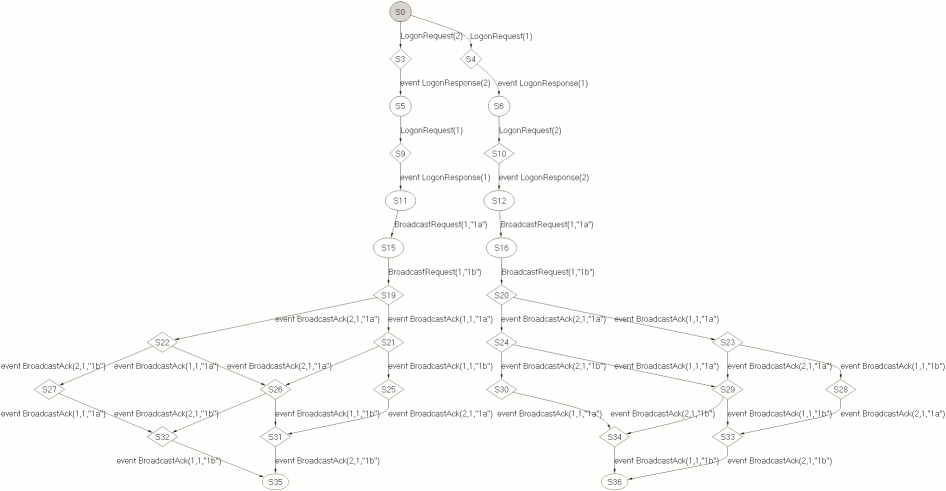
\includegraphics[width=1\textwidth]{figures/Model_View_In_SpecExplorer.png}
					\caption{\label{Fig:Model_View_In_SpecExplorer} Visual Representation of Model in Spec Explorer \cite{SpecExplorer_ModelView}}
\end{figure}

\par
If an \acrshort{fsm} is created with a large or even infinite state space, a technique called \textit{Slicing} is used for generating smaller subsets of the full behavior models which are more suitable for testing.

\par
One of the examples for usage of Spec Explorer in practice is provided by Silva et. al. \cite{Silva_SpecExplorer} where they apply it together with \textit{ConcurTaskTrees}. They create task models using the ConcurTaskTrees notation
and use a tool TERESA for generating \acrshort{fsm} from it. For creating the Spec\# model, the generated \acrshort{fsm} is given as an input to a tool called TOM (Task to Oracle Mapping tool) which was developed in scope of that research. The last step involves the generation of tests from the Spec\# models using Spec Explorer and mapping the generated tests to a test driver which then executes tests against the \acrshort{aut}.

\subsection{NModel}
\par
NModel is a modeling framework based on the usage experiences of Spec Explorer. Unlike the Spec Explorer, which uses separate compiler for compiling Spec\# models, NModel uses the standard .NET v2.0 compiler. Modeling with NModel requires coding knowledge since models are required to be implemented using C\#.

\par
Based on the obtained model, NModel generates a \acrshort{fsm} or an \acrshort{efsm} which can later be traversed with different coverage criteria passed to modules responsible for the test generation.

\par
NModel is made up of multiple artifacts. The NModel library consists of attributes and data types for writing models. The Model Program Viewer (\texttt{mpv}) and the Model Program to Dot (\texttt{mp2dot}) modules are responsible for visualization and analysis of the created model. The Model Program Viewer is visualized in the figure below. The Offline Test Generator (\texttt{otg}) provides an opportunity to generate the test suite off-line. The Conformance Tester (\texttt{ct}) module can be used in both ways, off-line as well as on-line \acrshort{mbt}.

\begin{figure} [htbp!]
	\centering
					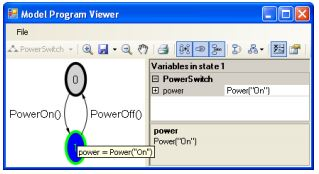
\includegraphics[width=0.5\textwidth]{figures/NModel_mpv.JPG}
					\caption{\label{Fig:NModel_mpv} Model Program Viewer of NModel}
\end{figure}


\par
We came across the usage of NModel in multiple case-studies. In one of them, Chinnapongse et. al. \cite{Chinnapongse_NModel} use NModel for testing \acrshort{gui} of The Armed Forces Health Longitudinal Tracking Application–Mobile (AHLTA-Mobile). The application is based on a Windows Phone platform containing multiple modules. In the scope of their research, a Military Acute Concussion Evaluation (MACE) module consisting of 8 different GUI Screens in tested. They begin with creating the mental model of the application first, which is later coded in C\#. The resulting artifact is an \acrshort{efsm} that is used to generate tests off-line. The last part involves executing the generated tests against the MACE module.
\par
Another user of NModel was Gabriel Kolawole \cite{Kolawole_NModel} who tested a \acrshort{gui} and functionality of the Moodle Mobile Application in his master thesis.

\subsection{MobiGUITAR}
\par
MobiGUITAR was introduced by a consortium  of researchers from the University of Naples Federico II and the University of Maryland. Their previous project, GUI ripping \cite{GUIripping}, was created for desktop applications and was based on \acrshort{efg}, but since mobile applications are very state sensitive, they changed their approach and created MobiGUITAR based on \acrshort{fsm}. Currently MobiGUITAR is limited to the android platform.

\par
The testing process with MobiGUITAR is divided into three phases: ripping, generating and executing. Ripping dynamically explores the application and creates a \acrshort{fsm} with the application states and events. An example of a generated \acrshort{fsm} can be seen in Figure \ref{Fig:MobiGuitar}.

\begin{figure} [htbp!]
	\centering
					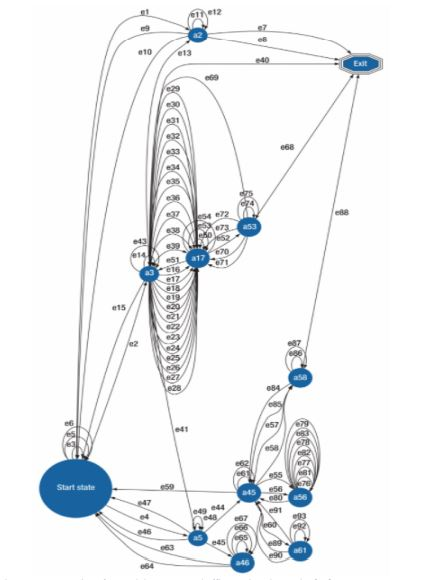
\includegraphics[width=0.5\textwidth]{figures/mobiguitar.JPG}
					\caption{\label{Fig:MobiGuitar} The abstract state machine for AardDict\cite{MobiGUITAR}}
\end{figure}

During the generation phase a \acrshort{fsm} is created along with a coverage criteria, such as pair-wise edge coverage to generate the test cases. This means that all the pairs of the adjacent edges are required to be taken together.
The execution phase applies a JUnit framework for testing the \acrshort{aut} returning the results to a tester. With these 3 phases together MobiGUITAR automates not only test generation and execution, but also the entire modeling process itself, which gives it an advantage over other \acrshort{mbt} tools.

\par
The main disadvantage of MobiGUITAR is its inability to perform functional testing. In \cite{MobiGUITAR}, it is mentioned that the tester can enhance the JUnit tests with assertions for detecting functional errors, but it still lacks features such as the ability to choose transitions based on background variables. For applications such as \acrshort{bsc}, verification of the functionality has the highest priority. MobiGUITAR is a great tool for verification of \acrshort{gui} correctness or robustness, but in our case, this falls short.

\subsection{Graphwalker}
\par
Graphwalker is an open-source tool for \acrshort{mbt} created by the developers at Spotify \cite{Spotify} and maintained by an open source community. Graphwalker takes the \acrshort{fsm} or the \acrshort{efsm} created with a set of predefined rules as an input and traverses it with a given coverage criterion.
The example input model can be observed in Figure  \ref{Fig:Graphwalker_model_example}.

\begin{figure} [htbp!]
	\centering
					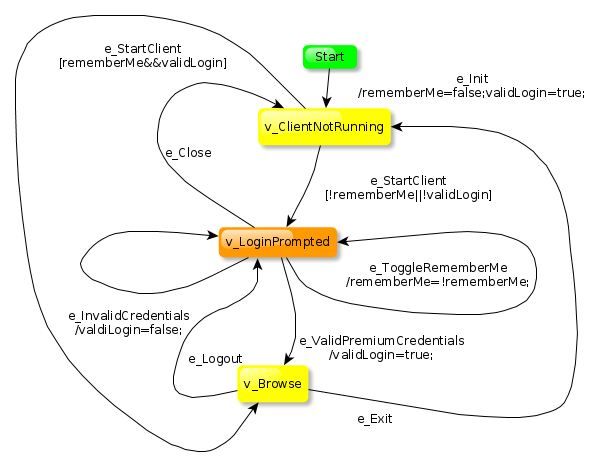
\includegraphics[width=0.8\textwidth]{figures/Graphwalker_model_example.png}
					\caption{\label{Fig:Graphwalker_model_example} Graphwalker input model example \cite{Graphwalker_Login_Example}}
\end{figure}

\par
The modeling currently needs to be done completely independent from the Graphwalker software. yEd Graph Editor \cite{yEd} is a tool suggested for creating models for Graphwalker and the developers are working on producing an internal modeling tool from the next release. Graphwalker supports off-line test generation, for which a basic knowledge of the command line interface is required by the user. The on-line test generation and execution is performed with tests written in Java or Python. 

\par
Graphwalker allows splitting models with shared steps. For example, when a model is huge and not readable, or if the user wants to separate a model into different functional parts of the system, they can annotate the vertex with a keyword \textit{shared}. This lets Graphwalker know while traversing that it can find the shared state in other models as well.

\par
The biggest advantage of the Graphwalker among the discussed modeling tools is that it has a very gentle learning curve for creating models and generating off-line tests from the created model. This allows testers to quickly adapt to the tool without undergoing any special training. Moreover, if test execution automation is not available, testers can execute generated tests manually against the \acrshort{aut}. We explore this later in this thesis.

\par
A couple of case-studies were encountered relating to the Graphwalker during the literature review, one of which described the application of \acrshort{mbt} using the Graphwalker in NASA's Goddard Mission Service Evolution Center (GMSEC) \cite{GMSEC}. The \acrshort{mbt} approach was applied to the \textit{software bus project} which was based on a \textit{pub-sub architecture}. Different applications could be connected using middle-ware wrappers which allowed them to publish/subscribe to different channels (also called \textit{topics}). As a result new bugs were found, which were not detected by the existing testing process. The paper contains a comparison between the effort and the results of using both \acrshort{fsm} and \acrshort{efsm}. It discusses some pitfalls of \acrshort{fsm} such as not being able to embed assertions in states leading to the inability to test different functionality. The usage of the legacy test cases were useful in resolving the specification ambiguity of the \textit{software bus project}. For instance in one of the cases the specification was describing a functionality that was not implemented at all and would result in wasteful modeling.

\subsection{USE}
\par
USE (\acrshort{uml}-based Specification Environment)  is a tool based on \acrshort{uml} modeling language enhanced with \acrshort{ocl} constraints. Its purpose is to assist analysts, designers and developers in executing the \acrshort{uml} models and checking the \acrshort{ocl} constraints. The system models, invariants,  pre- and post-conditions can be specified in a textual form. The models are defined in a \texttt{.use} file and generation of its instances is orchestrated by \texttt{.assl} file. The files with \texttt{.ins} extensions contain extra optional invariants. Generation of snapshots is done by the user through editing the \texttt{.assl} file. Figure \ref{Fig:USE_test_generation} shows the structure of an \texttt{.assl} file.

\begin{figure} [htbp!]
	\centering
					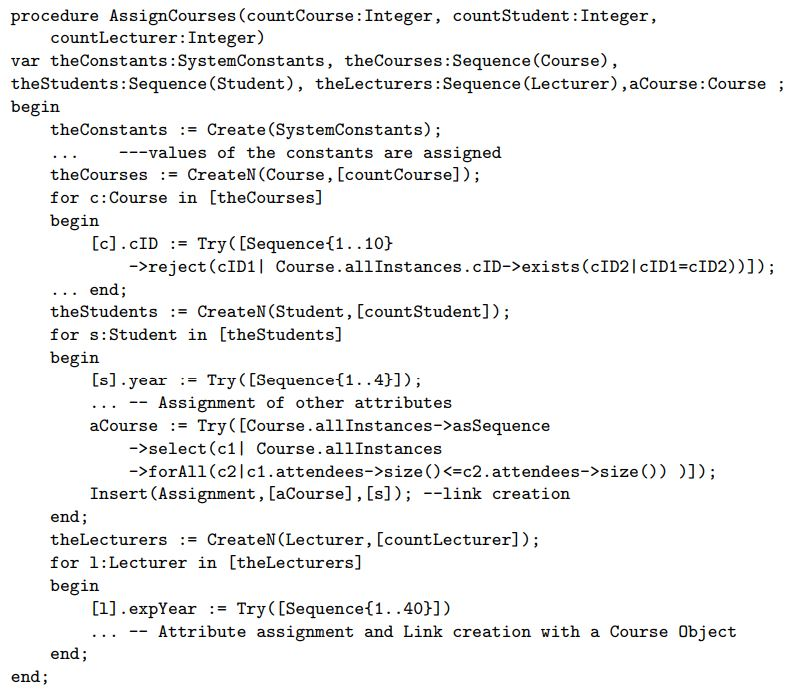
\includegraphics[width=0.8\textwidth]{figures/USE_test_generation.JPG}
					\caption{\label{Fig:USE_test_generation} Example of .assl file \cite{USE_Alloy_Z_comparison}}
\end{figure}

\par
One usage of the USE tools can be observed in \cite{USE_Alloy_Z_comparison} where it is compared to the other tools such as Alloy Analyzer, ProZ and Zlive in order to detect abilities and weaknesses of the tools used in different modelling languages. For this purpose, they conducted a simple experiment with a \textit{Course Assignment System}, which was written in 3 different modeling languages, \acrshort{uml} enhanced with \acrshort{ocl}, Alloy and Z. Then they used these different tools and compared their results with each other.

\subsection{Agile Requirements Designer from CA Technologies}
\par
Agile Requirements Designer is a \acrshort{mbt} tool commercially developed by CA Technologies. Models are represented in the form of flowcharts. It can be used for off-line as well as on-line execution. The example model could be observed in the figure \ref{Fig:AgileRequirementDesigner_Charts}. This model supports multiple coverage criteria such as coverage of all paths, all edges, all nodes and pairwise edge coverage.

\begin{figure} [htbp!]
	\centering
					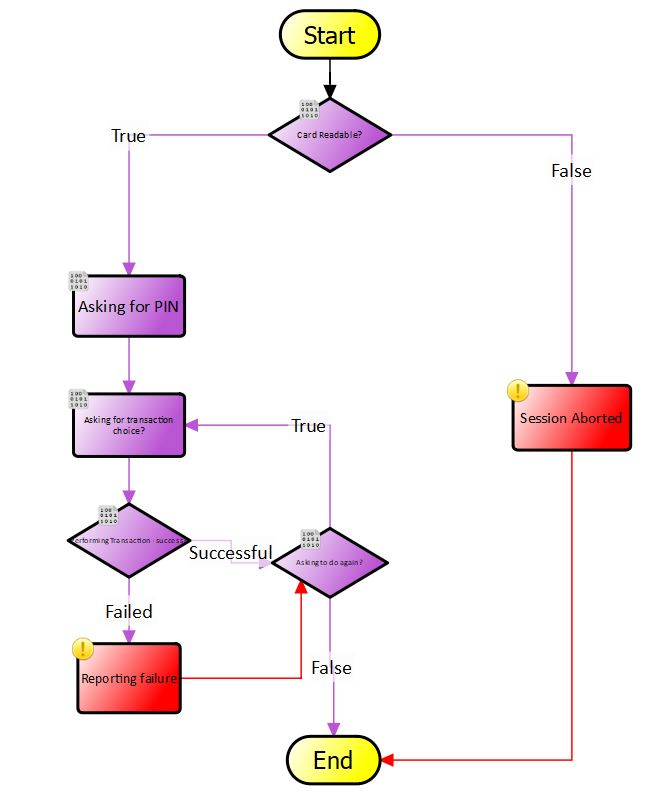
\includegraphics[width=0.8\textwidth]{figures/AgileRequirementDesigner_Charts.JPG}
					\caption{\label{Fig:AgileRequirementDesigner_Charts} Model in Agile Requirement Designer}
\end{figure}

\par
CA Technologies provide more tools for testing such as the CA Test Data Manager which, together with Agile Requirement Designer broadens the opportunities for providing high coverage during software testing. Agile Requirement Designer has integration interfaces to the popular issue tracker softwares such as Microsoft TFS, Atlassian Jira amongst others. These interfaces create opportunities to directly add or alter the generated test cases from models to an issue tracker software used by the companies. Agile Requirement Designer also provides interfaces for the popular test execution automation engines, such as Ranorex and others.

\par
To sum up, Agile Requirement Designer gives the opportunity to integrate \acrshort{mbt} into a company with less changes required for the current testing process. It would have been our first choice of selection, but unfortunately, we couldn't avail an answer to the request for using it in this thesis.

\section{Discussion}

\par
All the tools reviewed in the previous section were suitable for applying off-line \acrshort{mbt} for \acrshort{bsc} except MobiGUITAR which supports only the android platform. The criteria of evaluation for rest of the tools were based on the requirements given from Brainloop that the chosen tool should be usable for all the quality engineers within the company. We briefly examine the tools through this lens. The tool USE requires adoption of \acrshort{uml} as well as the fairly complex language for writing the generation criteria in \texttt{.assl} file, due to which we give it the least priority. NModel and Spec Explorer require the knowledge of programming languages and programming concepts which reduced their priority in our list as well. The remaining tools are CA Agile Requirement Designer and Graphwalker. They don't have a steep learning curve, as they don't require adoption of any new languages. For this reason they gain the highest priority in our list. CA Agile Requirement Designer gets a higher priority due to its interfaces to many other already used technologies at Brainloop, which was making it easier to integrate \acrshort{mbt} into the current testing process. Unfortunately, we were unable to acquire the permissions to use it in our thesis. As a result we chose Graphwalker, the next tool with the next highest priority. Table \ref{tab:Prioritized_Tools} summarizes the prioritization of underlying tools.

\begin{table}[]
    \centering
    \begin{tabular}{|l|l|p{8cm}|}
        \hline
        Priority & Tool & Reasons \\
        \hline
        1 & Graphwalker & Requires no programming knowledge for applying off-line \acrshort{mbt} \\
        \hline
        2 & CA Agile Requirement Designer & Easily integrable into Brainloops current testing process. Request for usage was not responded \\
        \hline
        3 & NModel & Requires programming knowledge \\
        \hline
        4 & Spec Explorer & Requires programming knowledge, Product is not maintained any more \\
        \hline
        5 & USE & Requires adoption of new languages for modeling and test generation\\
        \hline
        6 & MobiGUITAR & Supports only android platform \\
        \hline
    \end{tabular}
    \caption{Prioritized Tools}
    \label{tab:Prioritized_Tools}
\end{table}